%==============================================================================
% presentation.tex
%==============================================================================


%==============================================================================
% Configuration
%==============================================================================

% Internationalisation
\usepackage[utf8]{inputenc}
\usepackage[T1]{fontenc}
% \usepackage[ngerman]{babel}

% Miscellaneous packages
\usepackage{url}
\usepackage{color,listings,paralist}
\usepackage{enumerate}
\usepackage{tabularx}
\usepackage{alltt}
\usepackage{wasysym}
\usepackage{numprint}

% Use default Acrobat reader fonts
\usepackage{mathpazo}

% Use CM fonts (increases document size)
\usepackage{ae}

% Use images
\usepackage{graphicx}

% Configure beamer
\usetheme[secheader]{Ikhono}
\usefonttheme[onlylarge]{structurebold}
\setbeamertemplate{navigation symbols}{}

% Variables
\providecommand{\Title}{An Advanced Scheduler for Intervals}
\providecommand{\Subtitle}{Master's Thesis}
\providecommand{\Author}{Thomas Weibel <weibelt@ethz.ch>}
\providecommand{\Institute}{Laboratory for Software Technology, \\
  Swiss Federal Institute of Technology Z\"urich}
\providecommand{\Date}{September 7, 2010}

% PDF settings
\hypersetup{
  pdftitle={\Title, \Subtitle},
  pdfauthor={\Author},
  pdfsubject={\Institute},
  pdfkeywords={Master's Thesis, Thomas Weibel, Intervals, Parallel Programming}
}

% Titlepage
\title{\Title}
\subtitle{\Subtitle}
\author{\Author}
\institute{\Institute}
\date{\Date}

% Listings
\lstdefinestyle{Default}{
  language=Java,
  tabsize=2,
  mathescape=true,
  inputencoding=utf8,
  showstringspaces=false,
  fontadjust=true,
  basicstyle=\ttfamily,
  keywordstyle=\color{blue}\bfseries,
}
\lstset{style=Default}


%==============================================================================
% Document
%==============================================================================

\begin{document}


% Titlepage
\begin{frame}[plain]
  \titlepage
\end{frame}

\note{
  \begin{itemize}
  \item Hi and welcome to my talk.
  \item I'm going to present the work from my Master's thesis. The
    topic of my thesis was ``Advanced Scheduling for Intervals''.
  \end{itemize}

  Backup: Intervals are a new, higher-level primitive for
  multi-threaded programming allowing programmers to directly
  construct the program schedule. When using intervals, programmers
  create lightweight tasks and order them using \emph{happens before}
  relations. Programmers need not specify when tasks should block or
  acquire a lock. Instead they define when a task should execute in
  relation to other tasks, and what locks it should hold during
  execution. It is the duty of the runtime system to make this
  schedule pass. They are under active development at ETH Zürich as
  part of the PhD research of Niko.
}


\section*{Introduction}

\begin{frame}{Executive Summary}
  \begin{itemize}
  \item Advanced work-stealing scheduler for intervals
    \begin{itemize}
    \item[$\rightarrow$] Locality-aware scheduling using locality
      hints provided by the programmer
    \end{itemize}
  \item Providing locality hints to intervals is optional
    \begin{itemize}
    \item[$\rightarrow$] Performance of locality-ignorant programs
      executed with the new scheduler implementation is comparable to
      the original scheduler
    \end{itemize}
  \item Locality hints improve runtime and cache hit and miss rates
    \begin{itemize}
    \item[$\rightarrow$] \emph{Best locality} placement achieves up to
      $1.15\times$ speedup over \emph{worst} or \emph{ignorant
        locality} placement
    \item[$\rightarrow$] Cache hits are increased by up to $1.5\times$
      and cache misses are reduced by up to $3.1\times$
    \end{itemize}
  \end{itemize}
\end{frame}

\note{ 
  \begin{itemize}
  \item In my thesis we implemented and analyzed an advanced scheduler
    for intervals which is designed for locality-aware scheduling
    using locality hints provided by the programmer.
  \item Providing locality hints to intervals is optional and the
    performance of locality-ignorant programs executed with the new
    scheduler implementation is comparable to that of the original
    scheduler.
  \item We studied the performance of our new scheduler implementation
    with benchmarks using data sharing intervals. Our experimental
    results show that \emph{best locality} placement of intervals
    achieves up to 15 percent speedup over \emph{worst} or
    \emph{ignorant locality} placement. Cache hits are increased by up
    to 50 percent and cache misses are reduced by up to 310 percent.
  \end{itemize}
}

\begin{frame}{Work-Stealing Intervals Scheduler}
  \begin{itemize}
  \item Employs a fixed number of worker threads
  \item Each worker has a local deque to maintain its own pool of
    ready intervals:
    \begin{itemize}
    \item Puts and takes intervals to execute at the tail of its deque
    \item When its deque is empty, tries to steal an interval from the
      deque's head of a victim worker chosen at random
    \end{itemize}
  \item Reduces contention by having owner and thieves working on
    opposite sides of the deque
    \begin{itemize}
    \item Owner manipulates its deque in a LIFO (stack-like) manner
    \item Stealing operates in a FIFO manner
    \end{itemize}
  \end{itemize}
\end{frame}

\note{
  \begin{itemize}
  \item The implementation of intervals makes use of a work-stealing
    scheduler similar to those found in Cilk or Java 7.
  \item The work-stealing intervals scheduler employs a fixed number
    of threads called workers.
  \item Each worker has a local double-ended queue to maintain its own
    pool of ready intervals:
    \begin{itemize}
    \item When assigning a new interval to a worker, the worker puts
      it onto the tail of its deque. And when obtaining work, it takes
      a ready interval from the tail of its deque to execute.
    \item When a worker's deque is empty, it tries to steal an
      interval from the deque's head of a victim worker chosen at
      random. If the victim's deque is empty, then the thief picks
      another victim worker until it finds a victim whose deque it not
      empty.
    \end{itemize}
  \item Work-stealing scheduling reduces contention by having owner
    and thieves working on opposite sides of the deque: 
    \begin{itemize}
    \item As long as a worker's deque is not empty, the worker
      manipulates its deque in a stack-like manner.
    \item And since steals take place at the head of the victim's
      deque, stealing operates in a FIFO manner.
    \end{itemize}
  \end{itemize}
}

\begin{frame}{Locality-Aware Intervals Scheduling}
  \begin{itemize}
  \item Modern CMPs feature heterogeneous memory hierarchy:
    \begin{itemize}
    \item Access times depend on which processor an interval is
      running
    \item May be more efficient to run an interval on one processor
      than another
    \end{itemize}
  \item Locality-aware intervals can lead to improved performance:
    \begin{itemize}
    \item Data sharing intervals running on the same processor perform
      prefetching of shared regions for one another
    \item Running non-communicating intervals with high memory
      footprints on different processors reduces cache contention
    \end{itemize}
  \item Current work-stealing intervals scheduler is locality-ignorant
  \end{itemize}

  \begin{itemize}
  \item[$\Rightarrow$] Introduce LASSI\footnote{The correct acronym
      would be LASI but we chose LASSI instead as we really enjoy
      drinking refreshing masala lassi \smiley}, a locality-aware
    scheduler for intervals
  \end{itemize}
\end{frame}

\note{
  \begin{itemize}
  \item As modern chip multiprocessor systems feature a heterogeneous
    memory hierarchy where access times depend on which processor an
    interval is running, it may be more efficient to schedule an
    interval on one processor than another.
  \item Locality-aware intervals can lead to improved performance:
    \begin{itemize}
    \item By scheduling data sharing intervals on the same processor
      they perform prefetching of shared regions for one another.
    \item Scheduling non-communicating intervals with high memory
      footprints on different processors helps to reduce cache
      contention and potential cache capacity problems.
    \end{itemize}
  \item The current implementation of the intervals library uses a
    locality-ignorant work-stealing scheduler to schedule ready-to-run
    intervals.
  \item When using locality-ignorant work-stealing we cannot fully
    exploit the heterogeneous memory hierarchy of CMPs for our
    benefit. Thus, we implement and analyze LASSI, a locality-aware
    scheduler for intervals.
  \end{itemize}
}


\section{Approach}

\begin{frame}{Outline}
  \tableofcontents[current]
\end{frame}

\note{
  \begin{itemize}
  \item Before starting with the implementation of the new scheduler,
    we implement a synthetic multi-threaded locality-aware benchmark
    called \emph{Cache Stress Test}.
  \item This benchmark serves as a proof of concept for our plan to
    introduce locality-aware intervals:
    \begin{itemize}
    \item If a multi-threaded benchmark with best possible locality
      has better performance and fewer last-level cache misses than
      the same benchmark with another or no specific locality, we
      should be able to see the same effect when porting the benchmark
      to a locality-aware implementation of intervals.  
    \item Hence, we know whether it makes sense to design a
      locality-aware intervals scheduler.
    \end{itemize}
  \end{itemize}
}

\begin{frame}{Cache Stress Test}
  \begin{itemize}
  \item We wrote our benchmark for the Intel Nehalem system. The
    system has 2 processors with 4 cores each. Every core has its
    separate level 1 and 2 caches, but the per-processor 8 MB level 3
    cache is shared between all cores of the same processor.
  \item \emph{Cache Stress Test} first randomly initializes two
    integer arrays of size \numprint{2097144}, i.e. the size of each
    array is about 8 MB. This is equal to the size of the last level
    cache per processor. Then the benchmark creates 8 \emph{Cache
      Stress} threads per core with their affinity set to this
    specific core. Overall, we create 64 threads, bound to the 8 cores
    in groups of 8 threads. To bind threads to a specific core, we use
    the affinity library introduced later.
  \item One half of the threads operate on the elements of the first
    array and the other half operate on the elements of the second
    array. Each thread adds and multiplies all the elements of its
    respective array 100 times.
  \end{itemize}
\end{frame}

\note{
  \begin{itemize}
  \item Before starting with the implementation of the new scheduler,
    we implement a synthetic multi-threaded locality-aware benchmark
    called \emph{Cache Stress Test}. This benchmark serves as a proof
    of concept for our plan to introduce locality-aware intervals: If
    a multi-threaded benchmark with best possible locality has better
    performance and fewer last-level cache misses than the same
    benchmark with another or no specific locality, we should be able
    to see the same effect when porting the benchmark to a
    locality-aware implementation of intervals. Hence, we know whether
    it makes sense to design a locality-aware intervals scheduler.
  \item We wrote our benchmark for the Intel Nehalem system. The
    system has 2 processors with 4 cores each. Every core has its
    separate level 1 and 2 caches, but the per-processor 8 MB level 3
    cache is shared between all cores of the same processor.
  \item \emph{Cache Stress Test} first randomly initializes two
    integer arrays of size \numprint{2097144}, i.e. the size of each
    array is about 8 MB. This is equal to the size of the last level
    cache per processor. Then the benchmark creates 8 \emph{Cache
      Stress} threads per core with their affinity set to this
    specific core. Overall, we create 64 threads, bound to the 8 cores
    in groups of 8 threads. To bind threads to a specific core, we use
    the affinity library introduced later.
  \item One half of the threads operate on the elements of the first
    array and the other half operate on the elements of the second
    array. Each thread adds and multiplies all the elements of its
    respective array 100 times.
  \end{itemize}
}

\begin{frame}{Locality}
  We implement several different variants of the \emph{Cache Stress
    Test}, each having different locality properties:

  \begin{description}
  \item[Best Locality:] All the threads working on the first array
    have affinity for a core on the first processor and all threads
    working on the second array have affinity for a core on the second
    processor.
  \item[Ignorant Locality:] The threads are not bound to any specific
    core, i.e. they are \emph{ignorant} of their locality.
  \item[Random Locality:] The affinity of the threads is set to a
    \emph{random} core.
  \item[Worst Locality:] Half the threads with affinity for a core on
    the first processor work on the first array, and the other half
    works on the second array and vice versa.
  \end{description}
\end{frame}

\note{
  We implement several different variants of the \emph{Cache Stress
    Test}, each having different locality properties:

  \begin{description}
  \item[Best Locality:] All the threads working on the first array
    have affinity for a core on the first processor and all threads
    working on the second array have affinity for a core on the second
    processor.
  \item[Ignorant Locality:] The threads are not bound to any specific
    core, i.e. they are \emph{ignorant} of their locality.
  \item[Random Locality:] The affinity of the threads is set to a
    \emph{random} core.
  \item[Worst Locality:] Half the threads with affinity for a core on
    the first processor work on the first array, and the other half
    works on the second array and vice versa.
  \end{description}
}

\begin{frame}{Best and Worst Locality}
  \begin{columns}[c]
    \begin{column}{0.50\textwidth}
      \begin{center}
        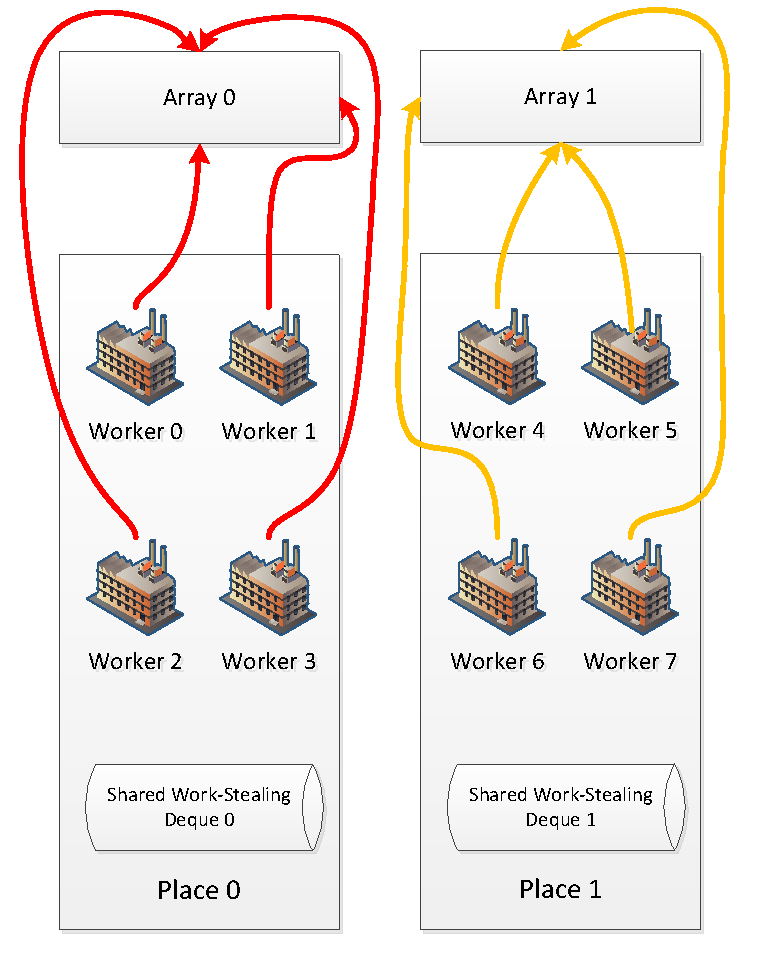
\includegraphics[width=\textwidth]{figures/cache-stress-test-mafushi-best} \\
        \tiny{Best Locality}     
      \end{center}
    \end{column}
    \begin{column}{0.50\textwidth}
      \begin{center}
        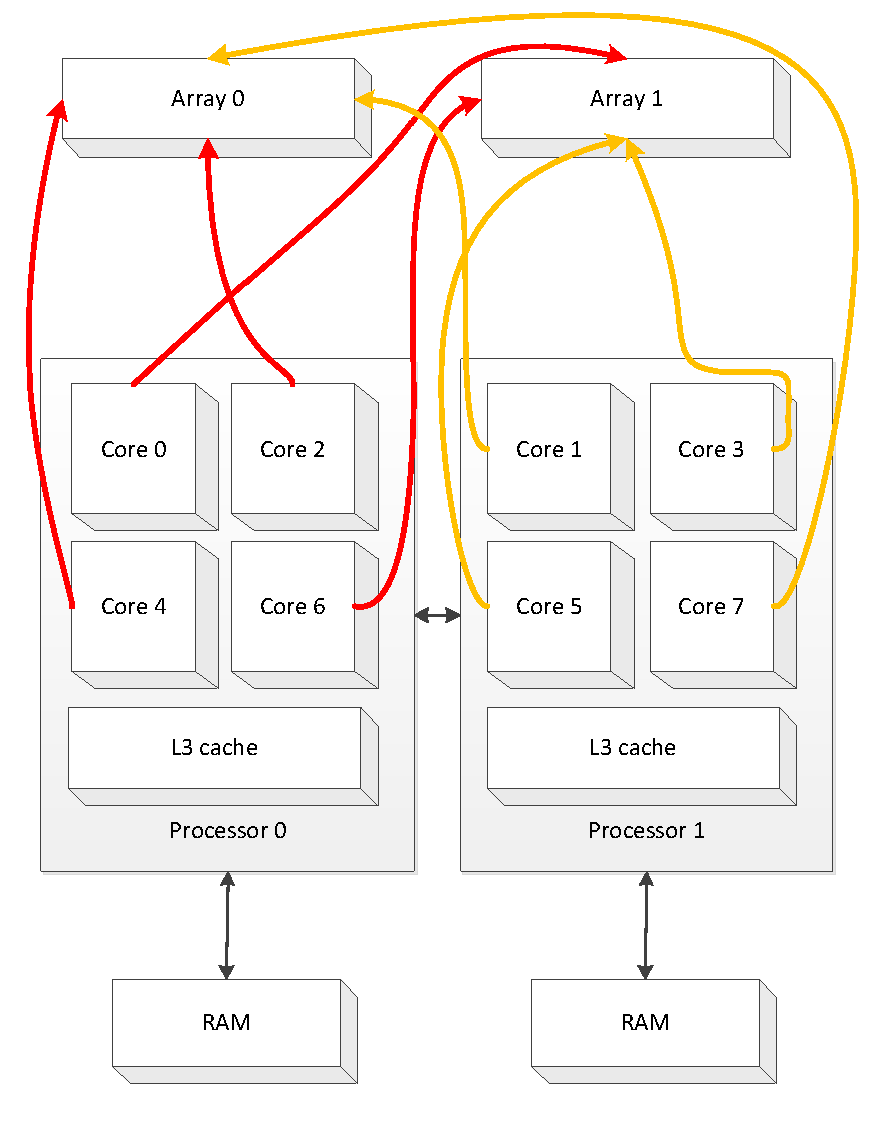
\includegraphics[width=\textwidth]{figures/cache-stress-test-mafushi-worst} \\
        \tiny{Worst Locality}
      \end{center}
    \end{column}
  \end{columns}
\end{frame}

\note{
}

\begin{frame}{Performance}
  TODO
\end{frame}

\note{
}

\begin{frame}{Performance}
  TODO
\end{frame}

\note{
}


\section{Implementation}

\begin{frame}{Outline}
  \tableofcontents[current]
\end{frame}

\note{
}

\begin{frame}{TODO}
  TODO
\end{frame}

\note{
}


\section{Performance Evaluation}

\begin{frame}{Outline}
  \tableofcontents[current]
\end{frame}

\note{
}

\begin{frame}{TODO}
  TODO
\end{frame}

\note{
}


\section{Related Work}

\begin{frame}{Outline}
  \tableofcontents[current]
\end{frame}

\note{
}

\begin{frame}{TODO}
  TODO
\end{frame}

\note{
}


\section{Conclusions and Future Work}

\begin{frame}{Outline}
  \tableofcontents[current]
\end{frame}

\note{
}

\begin{frame}{TODO}
  TODO
\end{frame}

\note{
}


\section*{Outro}

\begin{frame}{Summary}
  \begin{itemize}
  \item TODO
  \end{itemize}
\end{frame}

\note{
}

\begin{frame}
  \begin{center}
    \huge Questions?
  \end{center}
\end{frame}

\note{
}


\appendix

\section{Appendix}

\subsection{Work-Stealing Queue Implementations}

\begin{frame}{Introduction}
  \begin{itemize}
  \item The performance of work-stealing schedulers is in a large part
    determined by the efficiency of their work queue
    implementations. In the non-blocking work-stealing scheduler, the
    queues are implemented with non-blocking synchronization. That is,
    instead of using mutual exclusion, it uses atomic synchronization
    primitives such as Compare-and-Swap. The current work-stealing
    queue of intervals however uses mutual exclusion when trying to
    steal. Thus, as a separate effort, we design and explore
    alternative non-blocking queue implementations with the aim to
    improve work-stealing performance.
  \end{itemize}
\end{frame}

\note{
  \begin{itemize}
  \item The performance of work-stealing schedulers is in a large part
    determined by the efficiency of their work queue
    implementations. In the non-blocking work-stealing scheduler, the
    queues are implemented with non-blocking synchronization. That is,
    instead of using mutual exclusion, it uses atomic synchronization
    primitives such as Compare-and-Swap. The current work-stealing
    queue of intervals however uses mutual exclusion when trying to
    steal. Thus, as a separate effort, we design and explore
    alternative non-blocking queue implementations with the aim to
    improve work-stealing performance.
  \end{itemize}
}

\begin{frame}{Conclusions}
  \begin{itemize}
  \item TODO
  \end{itemize}
\end{frame}

\note{
}

\begin{frame}{Future Work}
  \begin{itemize}
  \item TODO
  \end{itemize}
\end{frame}

\note{
}

\subsection{Bibliography}

\begin{frame}
  \begin{thebibliography}{10}
    % Articles
    \beamertemplatearticlebibitems

  \bibitem{data-locality} Umut A. Acar et al. {\em``The data locality
      of work stealing''}. 2000.

  \bibitem{ws-sched} Robert D. Blumofe and Charles
    E. Leiserson. {\em``Scheduling multithreaded computations by work
      stealing''}. 1999.

  \bibitem{cilk} Robert D. Blumofe et al. {\em``Cilk: an efficient
      multithreaded runtime system''}. 1995.

  \bibitem{slaw} Yi Guo et al. {\em``SLAW: a scalable locality-aware
      adaptive work-stealing scheduler for multi-core
      systems''}. 2010.

  \bibitem{java-fork-join} Doug Lea. {\em``A Java fork/join
      framework''}. 2000.

  \bibitem{intervals} Nicholas D. Matsakis and Thomas
    R. Gross. {\em``Programming with Intervals''}. 2009.

  \bibitem{cache-locality} James Philbin et al. {\em``Thread
      scheduling for cache locality''}. 1996.

  \bibitem{cache-affinity} M. S. Squillante and
    E. D. Lazowska. {\em``Using Processor-Cache Affinity Information
      in Shared-Memory Multiprocessor Scheduling ``}. 1993.

  \end{thebibliography}
\end{frame}

\note{
  Those are a few selected references I used in my work.
}

\end{document}
